\section{Hipótesis y resultados}
Dado que la norma social se cumple, al menos para la vestimenta y las habilidades, esta sección estudia cómo responden los participantes al observar diferentes combinaciones de expresiones de género en su pares.

\subsection{Hipótesis}
\begin{hyp}
Cuando una persona no cumple la norma social o no es claro que la cumpla, la disposición a interactuar con esa persona es menor a si sí cumpliera la norma social. 
\end{hyp}

Dado que, en promedio, sí se cumple que las personas de identidad binaria se adhieran a la norma social, la primera predicción es que cuando las expresiones de género no señalizan claramente la identidad de género, la disposición a interactuar con esa persona va a ser más baja que si sus expresiones señalizaran claramente la identidad. Es decir, si una persona tiene una expresión de género femenina y otra masculina, la disposición de otros a interactuar con esa persona va a ser más baja a que si todas sus expresiones fueran femeninas o todas masculinas. Esta hipótesis sugiere que el costo de no interactuar es menor al costo esperado de que la persona esté violando la norma social ($\mathbb{P}$). 

\begin{hyp}
Las normas sociales y la disposición a interactuar varía entre identidades de género.
\end{hyp}

La literatura no ha explorado cómo el género de las personas se correlaciona con cómo responden a las normas sociales al momento de decidir interactuar con otros. Sin embargo, sí ha estudiado diferencias de comportamiento entre sexos en el juego del ultimátum (negociación), aunque los efectos que han encontrado son mixtos \citep{solnick2001genderultimatumgame, eckel2001chivalryultimatumgame, gomez2018gendernegociacion}.\footnote{\cite{solnick2001genderultimatumgame} encuentran que los hombres atraen mayores ofertas; mientras \cite{eckel2001chivalryultimatumgame} y \cite{gomez2018gendernegociacion} no encuentran diferencias en las ofertas. \cite{solnick2001genderultimatumgame} y \cite{gomez2018gendernegociacion} encuentran que los hombres rechazan más las ofertas de los hombres; mientras que \cite{eckel2001chivalryultimatumgame} encuentra que los hombres aceptan más las ofertas de las mujeres.} 

A pesar de que en el modelo las normas sociales son percibidas de igual manera por todos los jugadores, independiente de su identidad, la siguiente predicción es que la manera en que responden a las normas sociales varia entre géneros. Esto es que el costo de ver que se viola la norma social ($\theta$) es diferente entre identidades de género para cada combinación de expresiones de género que observe. Es decir el costo que percibe una persona de identidad femenina de ver que una persona de identidad masculina rompe la norma social es diferente al de ver a una persona de identidad no binaria romper la norma social. Estos, a su vez son diferentes a los costos que percibe una persona de identidad masculina o de identidad no binaria. Dados los límites de la literatura y del modelo, 
esta hipótesis se limita a esperar diferencias en la magnitud en la que responden personas de diferentes identidades al momento de elegir con quién interactuar. 

\begin{hyp}
Las personas que se adhieren a la norma social están menos dispuestas a interactuar con las personas que no cumplan la norma social. 
\end{hyp}

En el modelo, el jugador con identidad percibe el costo de violar la norma social, mientras que el otro jugador percibe el costo de interactuar con alguien que viola la norma social. Por el contrario, en el experimento los participantes enfrentaban ambos costos. La tercera predicción es que aquellas personas que cumplen la norma social están menos dispuestas a interactuar con una persona que señaliza estar violando la norma social. Esto es que si una persona percibe un costo alto de violar la norma social ($\xi$), también percibe un costo alto de interactuar con alguien que viola la norma social ($\theta$). Esto no quiere decir que todas las personas que se adhieren a la norma social lo hacen porque perciban un costo alto de violar la norma social, porque lo pueden hacer por la utilidad intrínseca que les genere esas expresiones; pero, sí supone que las personas que tienen un costo alto de violar la norma social, la cumplen.

\subsection{Estrategia empírica}
Para estimar cómo cambia la disposición a interactuar con una persona cuando cambia el conjunto de expresiones de género de esa persona, la información relevante es el orden que ocupó la persona $j$ cuando la persona $i$ organizó los perfiles y las características reportadas de la persona $j$.

Sea $Ranking_{ij}$ el orden inverso que la persona $i$ le asigna a la persona $j$, de manera que un valor más alto en \textit{Ranking} implica que la persona $i$ prefería trabajar con la persona $j$ por encima a las personas con menor \textit{Ranking} que $j$. Sea $vestimenta_j$ el puntaje estandarizado de qué tan femenina o masculina es la vestimenta que la persona $j$ eligió, donde un puntaje más alto implica que la vestimenta fue clasificada como más femenina. Sea $habilidad_j$ un indicador que toma el valor de uno si la  persona $j$ reporta ser más hábil comunicándose que en matemáticas. Sea $aspiracion_j$ un indicador que toma el valor de uno si la aspiración principal de la persona $j$ es familiar. Sean $edad_j$ la edad que reporta la persona $j$, $bogota_j$ un indicador de si la persona $j$ nació en Bogotá, $posicion\_inical_j$ el puesto que tenía la persona $j$ en la lista de la persona $i$ antes de que la persona $i$ reorganizara los perfiles según su preferencia y sea $\gamma_i$ el efecto fijo de la persona $i$; el modelo principal es: 
\begin{equation}
    \begin{split}
	Ranking_{ij}=& \beta_1vestimenta_j +  \beta_2habilidad_j + \beta_3habilidad_j\times vestimenta_{j} \\
	+ & \beta_4aspiracion_j + \beta_5edad_j + \beta_6bogota_j + \beta_7posicion\_inicial_j+\gamma_i + \epsilon_{ij}
	\end{split}
\end{equation}
Los resultados principales, basados en la estimación por MCO\footnote{El Apéndice C presenta las estimaciones por Logit rankeado y ordenado, y la estimación utilizando el \textit{ranking} promedio que recibió la persona $j$ entre todas las personas que observaron ese perfil.} de la Ecuación 1, consisten en las pruebas de hipótesis de si existe diferencia entre el \textit{ranking} esperado de una persona con todas sus expresiones masculinas (femeninas) con el \textit{ranking} esperado de cada una de las demás combinaciones de expresiones de género. Por ejemplo, una de las pruebas de hipótesis es si existe una diferencia entre el \textit{ranking} esperado de una persona con vestimenta femenina y que considera ser más hábil comunicándose (todas las expresiones femeninas) y el \textit{ranking} esperado de una persona con vestimenta femenina, que considera ser más hábil en matemáticas. Para las pruebas de hipótesis una vestimenta muy femenina (muy masculina) está definida como una vestimenta con un puntaje 1.5 desviaciones estándar arriba (abajo) de la media.

Para evaluar la Hipótesis 2, la Ecuación 1 fue estimada incluyendo la interacción del género de quien ordena los perfiles (la personas $i$, en adelante el \textit{ranker}) con las combinaciones de las expresiones de género. Luego, a partir de esa estimación, el \textit{ranking} que le da un \textit{ranker} femenino  a cada combinación de expresiones de género, es comparado con el que le da un \textit{ranker} masculino. También son comparados el \textit{ranking} esperado de una persona con todas sus expresiones femeninas (masculinas) con el \textit{ranking} esperado de las demás combinaciones de expresiones, cuando el \textit{ranker} es femenino y cuando es masculino. 

Para evaluar la Hipótesis 3, primero se definió que una persona cumplía la norma social (en adelante \textit{compliers}) si: (i) su identidad era masculina, había elegido una de las tres vestimentas más masculinas y consideraba ser más hábil en matemáticas, o  (ii) su identidad era femenina, había elegido una de las tres vestimentas más femeninas y consideraba ser más hábil comunicándose. Luego, la Ecuación 1 fue estimada incluyendo la interacción del indicador de \textit{complier} con las combinaciones de expresiones de género. Con base en esa estimación, el \textit{ranking}  que le da un \textit{complier} a cada combinación de expresiones de género es comparado con el que le da un no \textit{complier}. También son comparados el \textit{ranking} esperado de una persona que señaliza que cumple la norma social con el \textit{ranking} de las demás combinaciones de expresiones de género, cuando organiza los perfiles un \textit{complier} y cuando lo hace un no \textit{complier}. 

\subsection{Resultados}
Esta sección presenta los resultados del experimento. Estos resultados son sugestivos dado que para el tamaño de la muestra no hay poder para detectar resultados significativos.\footnote{El Apéndice D contiene los cálculos de poder.}

En la población agregada, una persona con todas sus expresiones de género femeninas recibe el mejor \textit{ranking}. En general, existe una preferencia por trabajar con las personas que reportan ser más hábiles comunicándose. Esta preferencia posiblemente se debe a que para el desarrollo de la tarea había un beneficio marginalmente mayor  de tener habilidades de comunicación. 

Lo que resulta interesante es que dentro de las personas cuya habilidad principal era la comunicación, las personas con una vestimenta femenina recibieron un \textit{ranking} 0.06d.e. más alto que las que tenían una vestimenta masculina. De manera similar, dentro de las personas que reportaron ser más hábiles en matemáticas, las personas que eligieron una vestimenta masculina, en promedio estuvieron 0.17d.e. más arriba en el \textit{ranking} que las personas con una vestimenta femenina. 

Por otra parte, en la población agregada, la diferencia entre el el \textit{ranking} que recibió una persona más hábil comunicándose y el \textit{ranking} que recibió una persona más hábil en matemáticas, aumenta a medida que la vestimenta es más femenina. Para una persona que eligió una vestimenta muy masculina, pasar de reportar como habilidad principal las matemáticas a reportar la comunicación aumentaba su \textit{ranking} en 0.1d.e. Mientras que para una persona con vestimenta muy femenina, pasar de reportar como habilidad principal las matemáticas a reporta la comunicación, aumenta su \textit{ranking} en 0.33d.e. 

\begin{table}[ht!]
    \centering
    \caption{Elección de pares a partir de expresiones de género}
    \label{tab:reg}
    \begin{threeparttable} \fontsize{8.5}{12}\selectfont {
    \begin{tabular}{lccccc} \hline \hline
                                                & \multicolumn{5}{c}{Ranker}                                                    \\\cmidrule{2-6}
                                                &   Todos   &  Femenino & Masculino & \textit{Complier} & No \textit{Complier}  \\ 
                                                &   (1)     &    (2)    &   (3)     &   (4)             & (5)                   \\ \hline
                                                &           &           &           &                   &                       \\
    Puntaje vestimenta                          &   -0.132  &   -0.344  &   0.035   &   -0.000	        &   -0.229              \\
                                                &   (0.207)	&   (0.312)	&   (0.280) &   (0.347)	        &   (0.266)             \\
    Habilidad comunicación                      &   0.497**	&   0.639*	&   0.322   &    0.286	        &   0.676**             \\
                                                &   (0.231)	&   (0.336)	&   (0.323) &   (0.372)	        &   (0.310)             \\
    Habilidad comunicación*Puntaje vestimenta   &   0.176	&   0.299	&   0.106   &    0.217	        &   0.153               \\
                                                &   (0.258)	&   (0.383)	&   (0.355) &   (0.414) 	    &   (0.351)             \\
    Aspiración familiar                         &   0.252	&   0.572*	&   -0.021  &    0.285	        &   0.225               \\
                                                &   (0.216)	&   (0.314)	&   (0.304) &   (0.301)	        &   (0.307)             \\
    Edad                                        &   0.001	&   -0.032	&   0.025   &    0.124	        &   -0.091              \\
                                                &   (0.064)	&   (0.091)	&   (0.093) &   (0.088)	        &   (0.091)             \\
    Bogotá = 1                                  &   -0.052	&   -0.160	&   0.023   &   -0.171	        &   0.125               \\
                                                &   (0.225)	&   (0.342)	&   (0.300) &   (0.314)	        &   (0.324)             \\
    Posición Inicial                            &  0.263***	&  0.263***	&  0.267*** &   0.368***    	&   0.178***            \\
                                                &   (0.046)	&   (0.066)	&   (0.065) &   (0.063)         &	(0.066)             \\
    Constante                                   &   2.873**	&   3.346*	&   2.564   &    0.107	        &   4.946**             \\
                                                &   (1.373)	&   (1.925)	&   (1.988) &   (1.895)	        &   (1.932)             \\
                                                &           &           &           &                   &                       \\
    Observaciones                               &   560     &   264     &   296     &   272             &   288                 \\
    Número de rankers                           &   70      &   33      &   37      &   34              &   36                  \\ \hline \hline
    \end{tabular}}
    \begin{tablenotes}
    \scriptsize{
    \item Nota: *** p$<$0.01, ** p$<$0.05, * p$<$0.1; errores estándar robustos en paréntesis.}
    \end{tablenotes}
    \end{threeparttable}
\end{table}

\begin{result}
Condicional en la habilidad, sugestivamente existe una mayor disposición a interactuar con las personas que señalizan que cumplen la norma social, especialmente cuando señaliza una identidad femenina. 
\end{result}

\begin{figure}[t!]
    \centering
    \label{fig:hypothesis_graphs}
    \caption{Ranking esperado por combinación de expresiones de género}
    \begin{minipage}{0.245\textwidth}
        
    \end{minipage}
    \begin{subfigure}{0.49\textwidth}
        \centering
        \caption{Todos}
        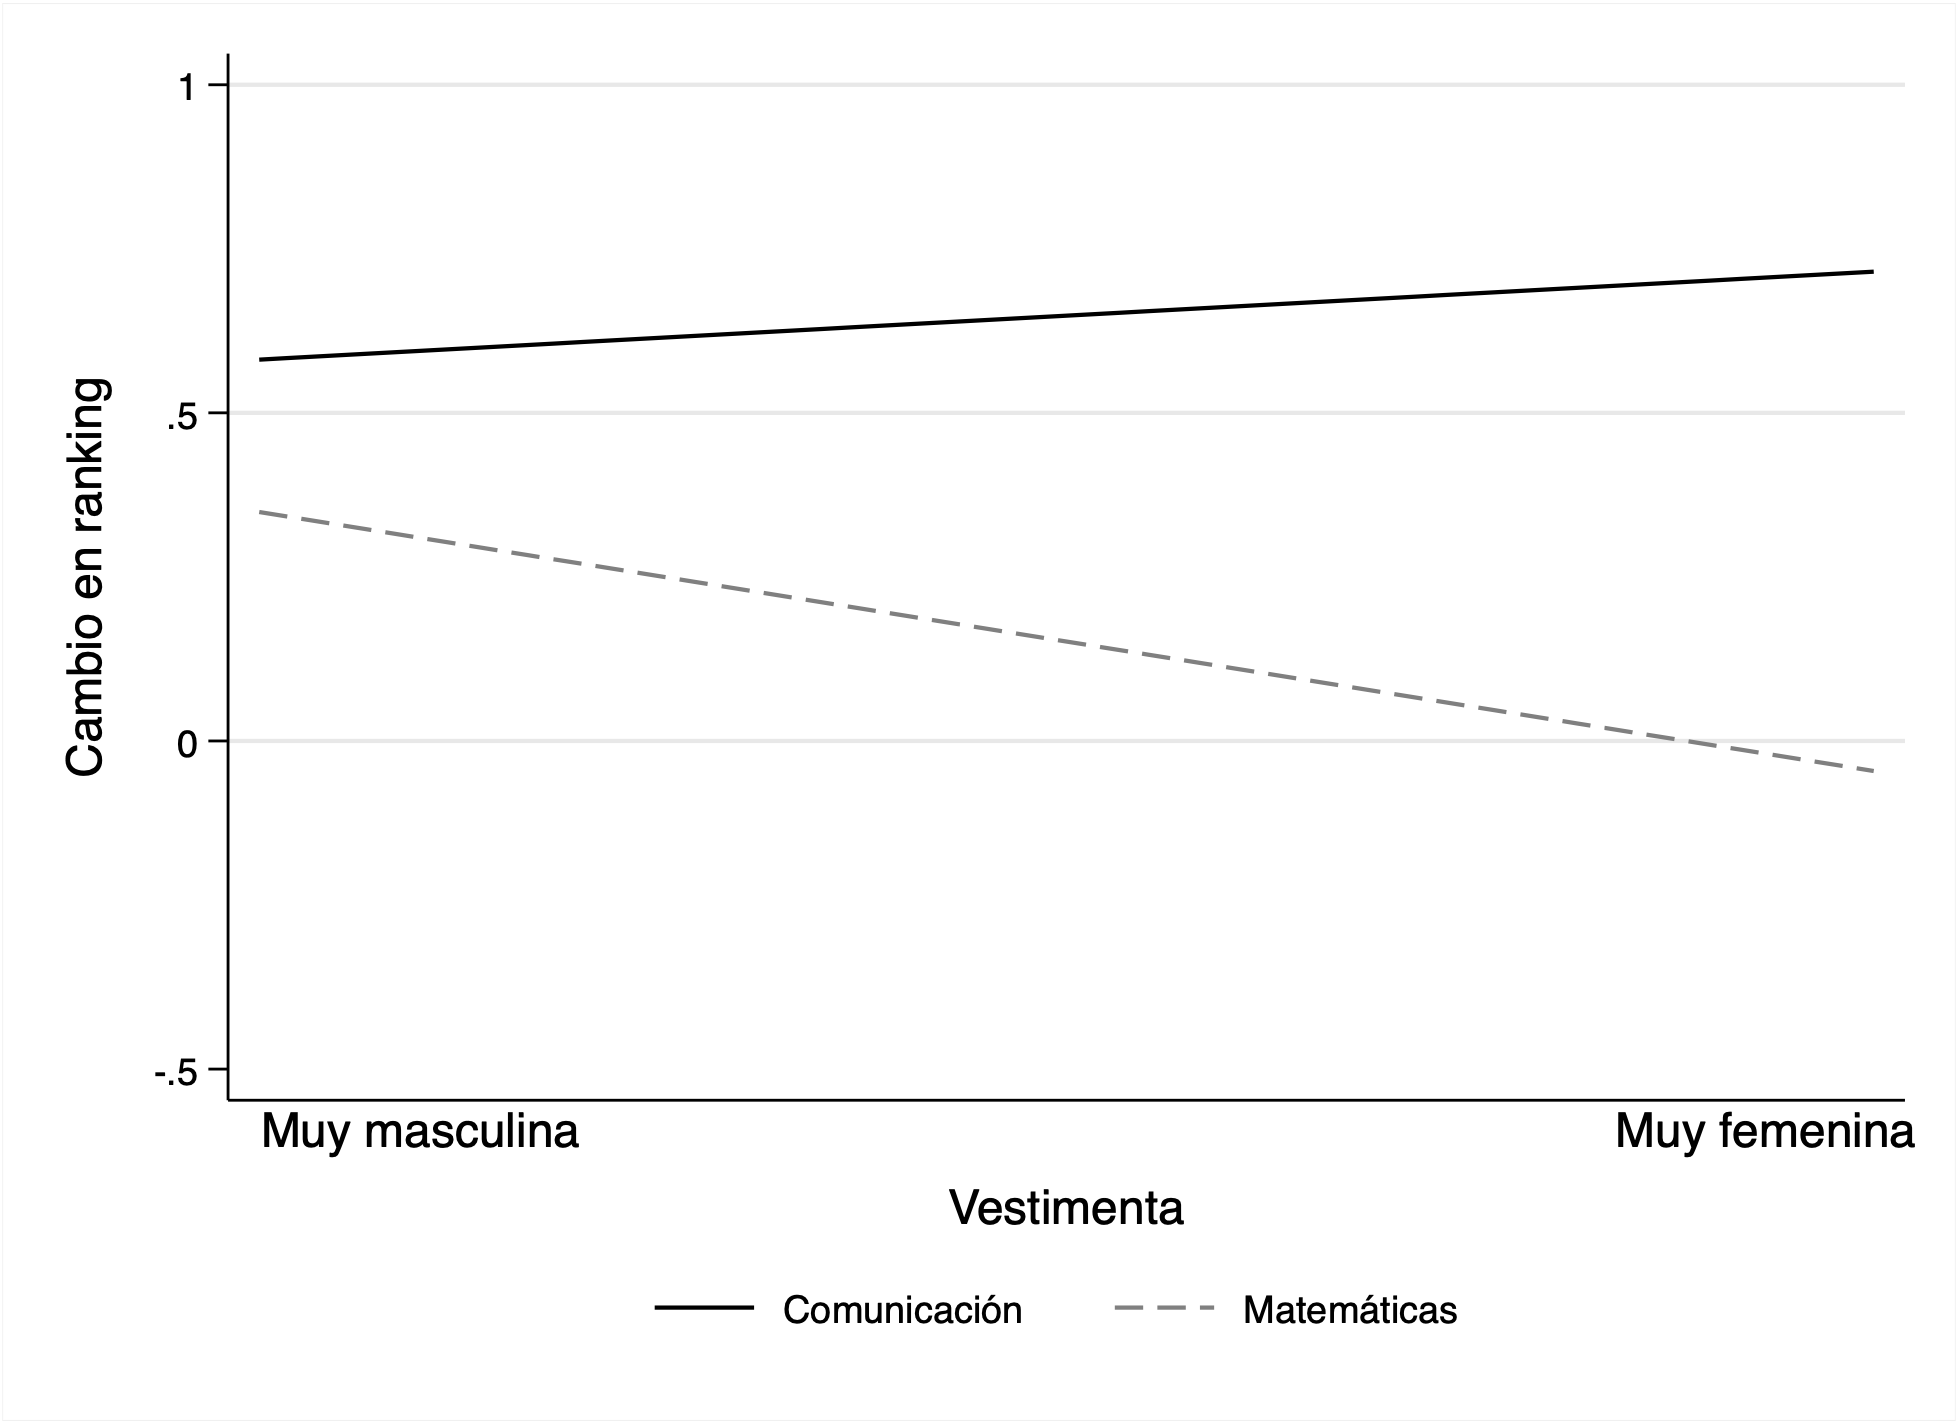
\includegraphics[width=7.8cm]{Images/h1_predicted_rank_score.png}
    \end{subfigure}
    \begin{minipage}{0.245\textwidth}
        
    \end{minipage}
    \centering
    \begin{subfigure}[t]{0.49\textwidth}
        \centering
        \caption{Rankers femeninos}
        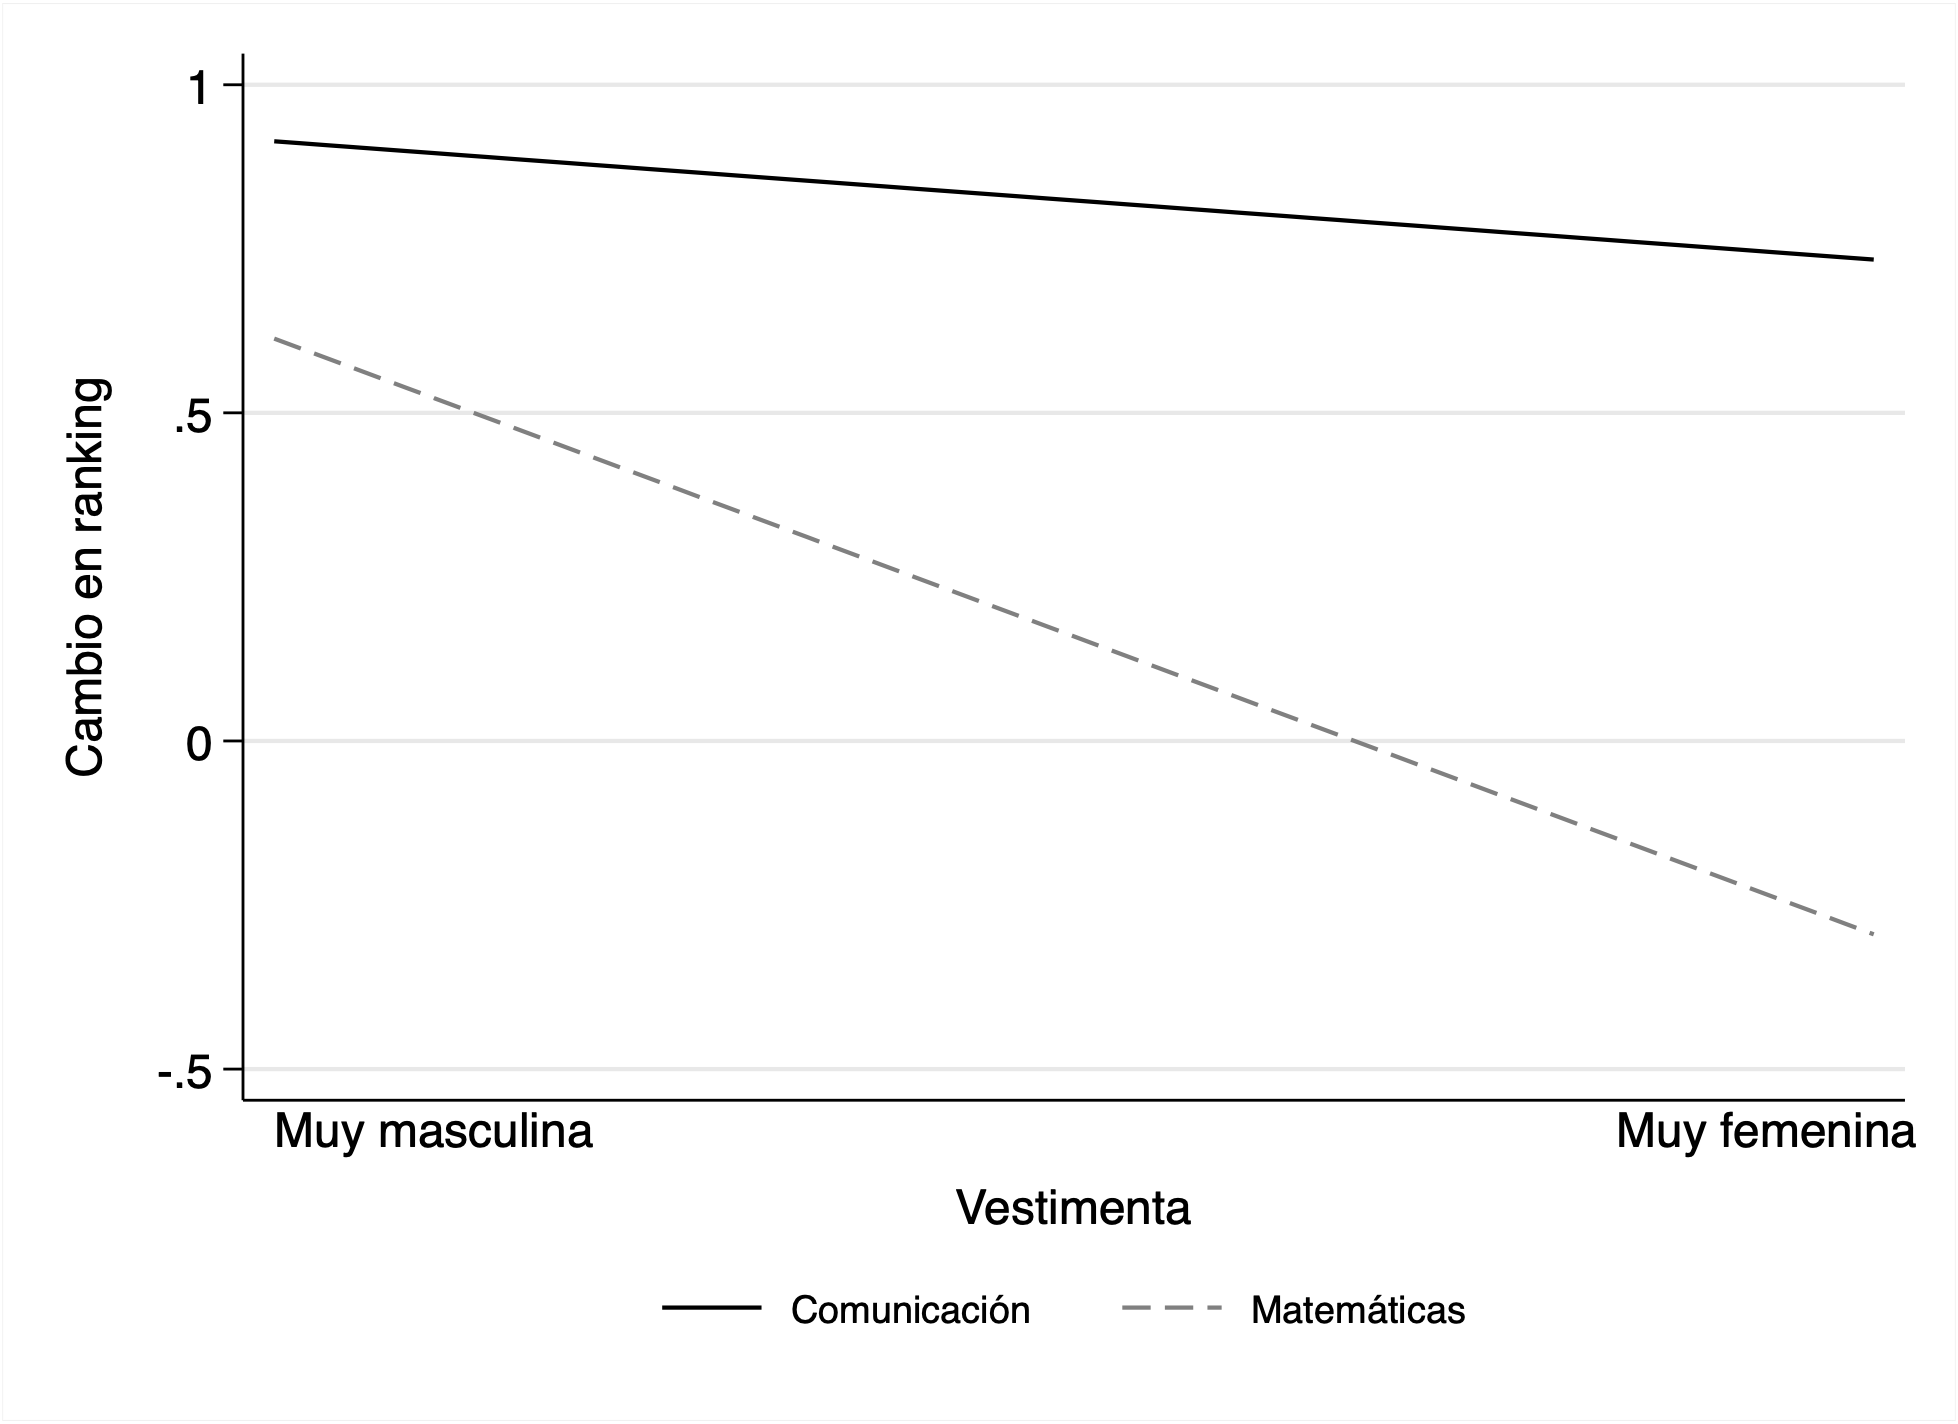
\includegraphics[width=7.8cm]{Images/h2_predicted_rank_score_fem.png}
    \end{subfigure}
    \begin{subfigure}[t]{0.49\textwidth}
        \centering
        \caption{Rankers masculino}
        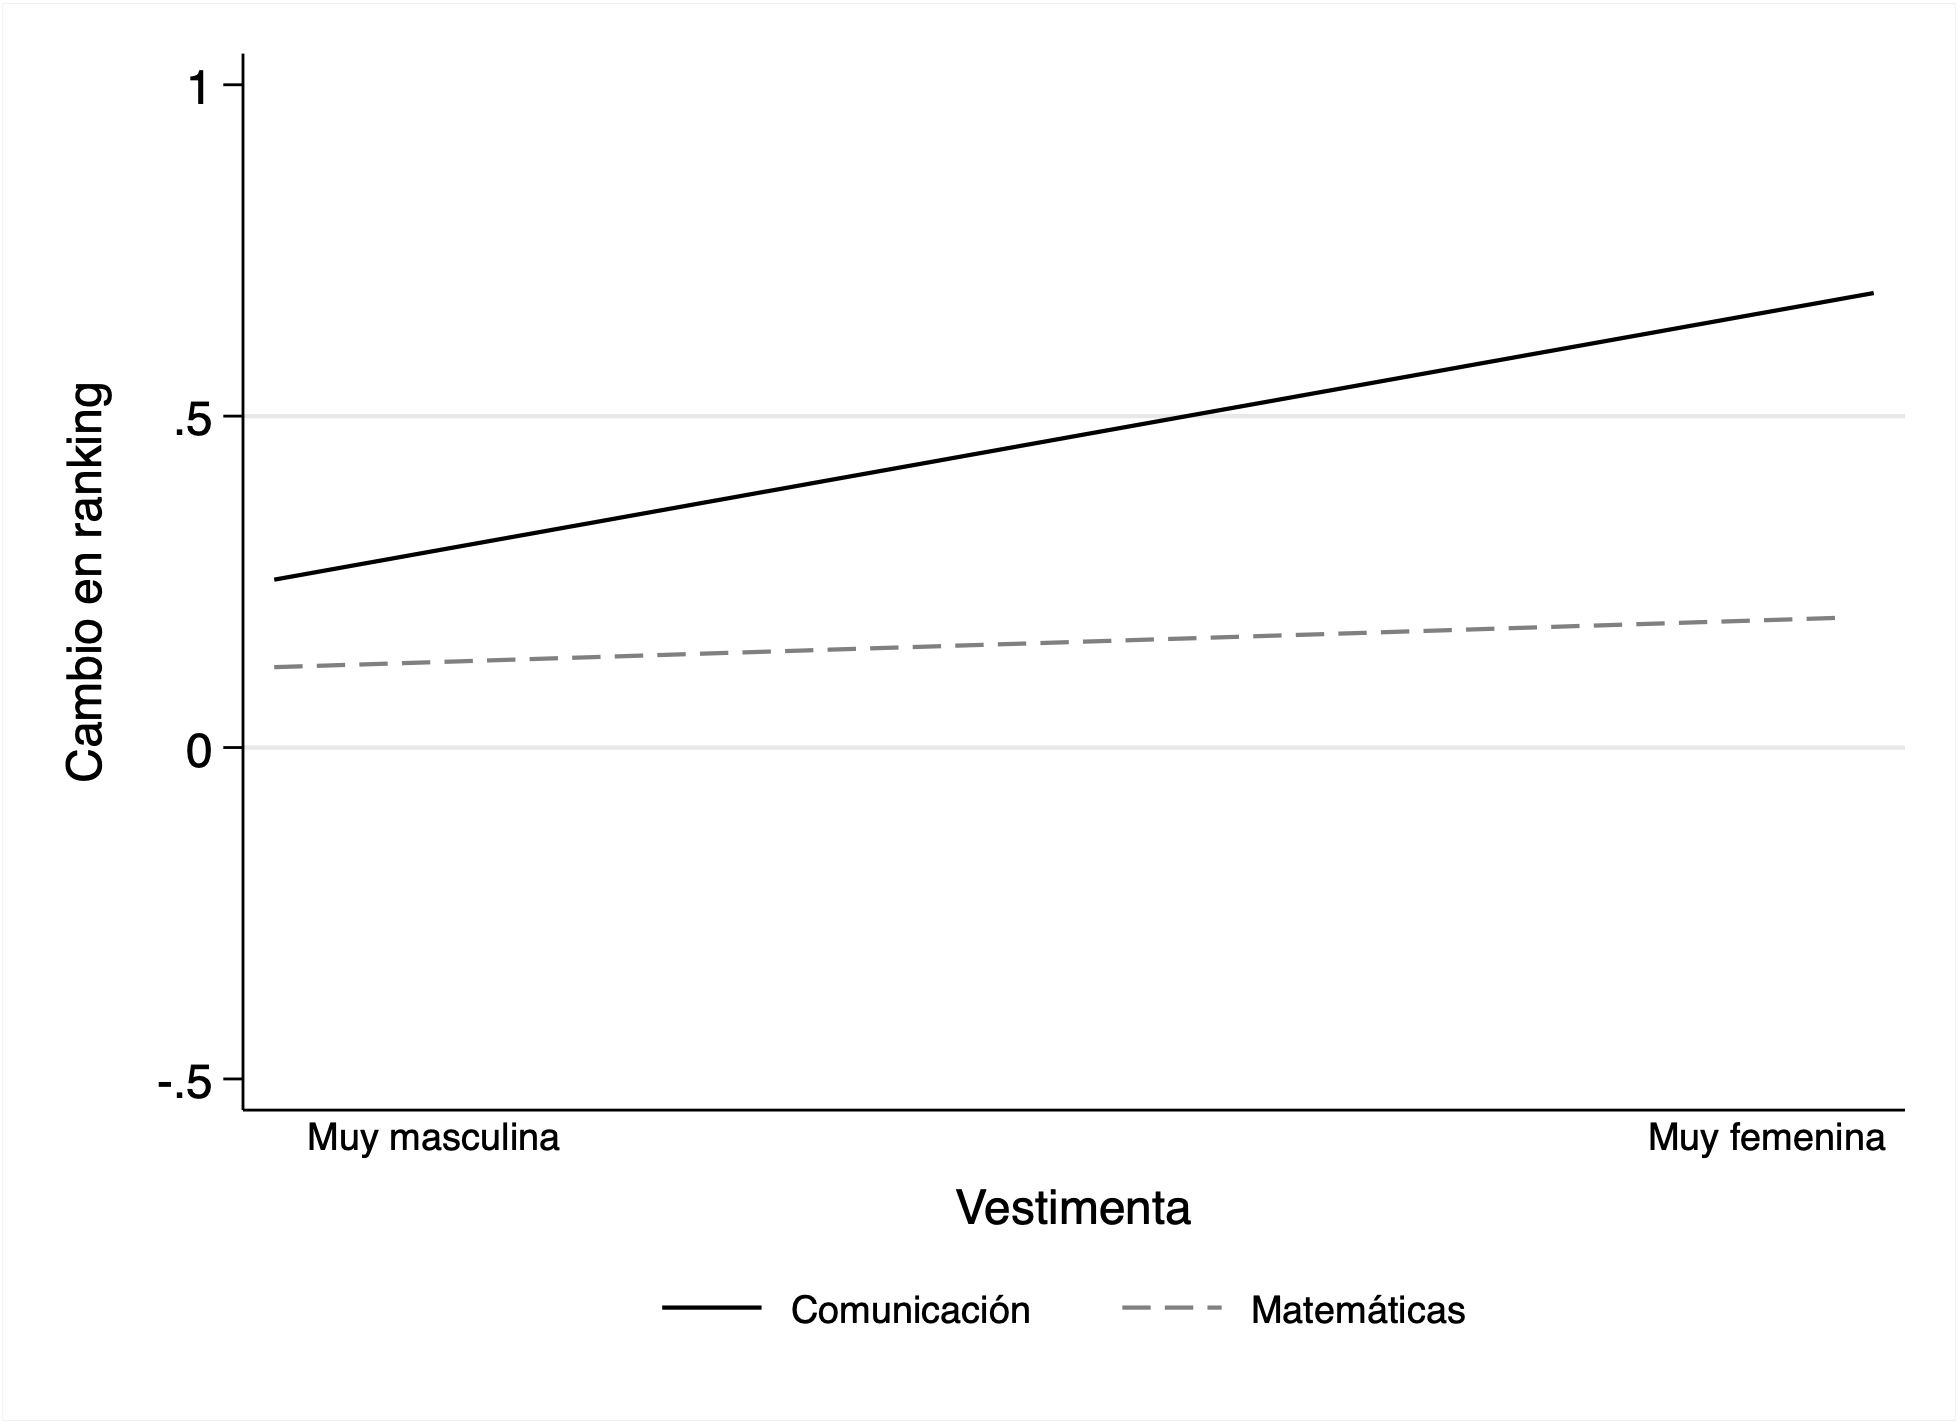
\includegraphics[width=7.8cm]{Images/h2_predicted_rank_score_masc.png}
    \end{subfigure}
    \begin{subfigure}[t]{0.49\textwidth}
        \centering
        \caption{Compliers}
        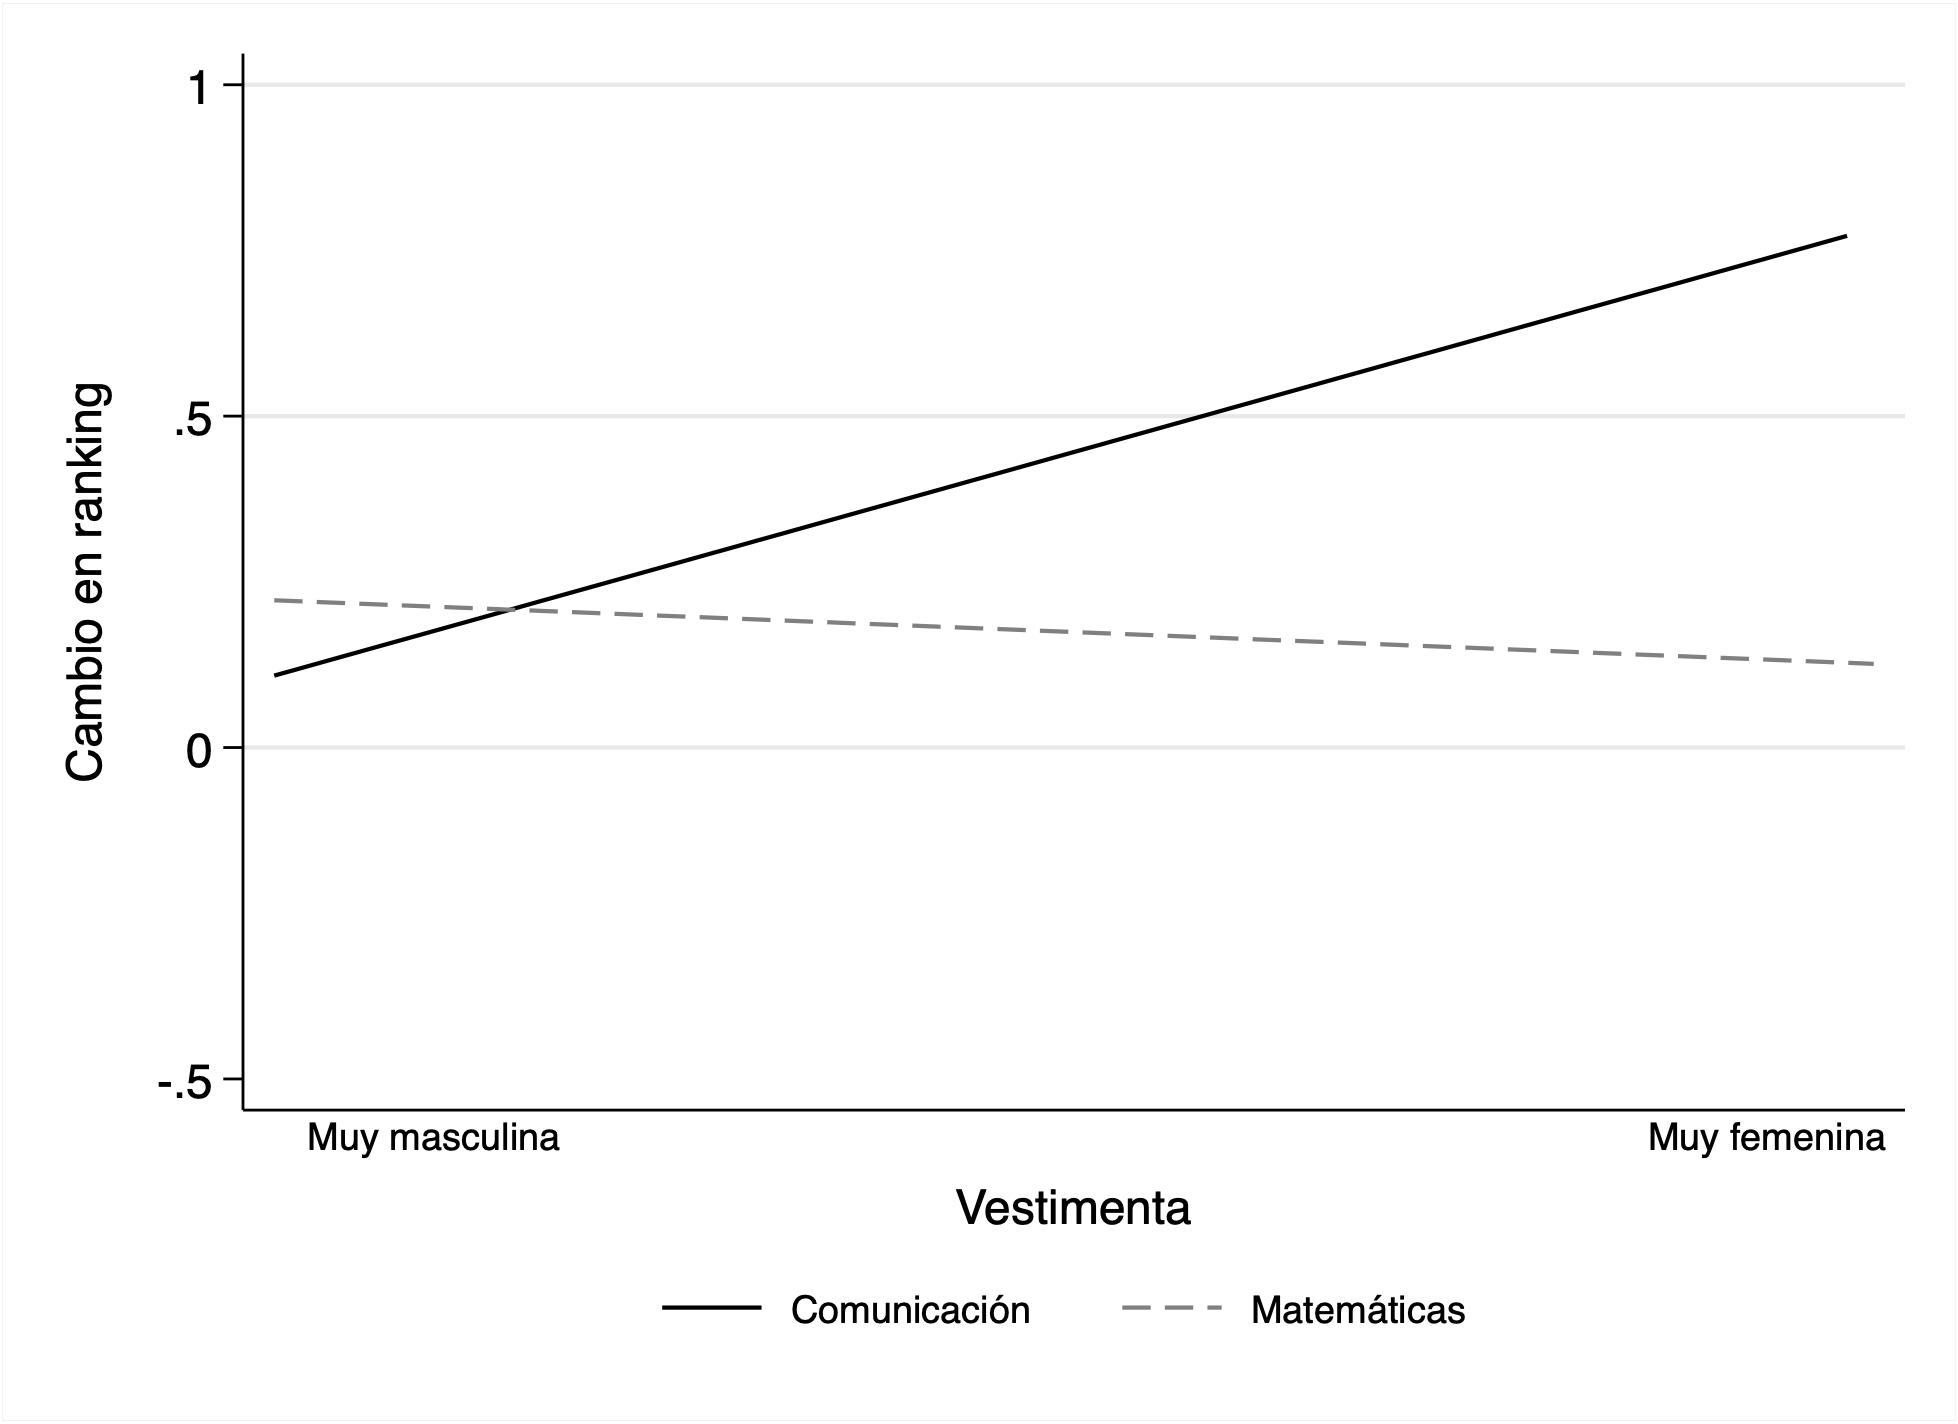
\includegraphics[width=7.8cm]{Images/h3_predicted_rank_score_complier.png}
    \end{subfigure}
    \begin{subfigure}[t]{0.49\textwidth}
        \centering
        \caption{No compliers}
        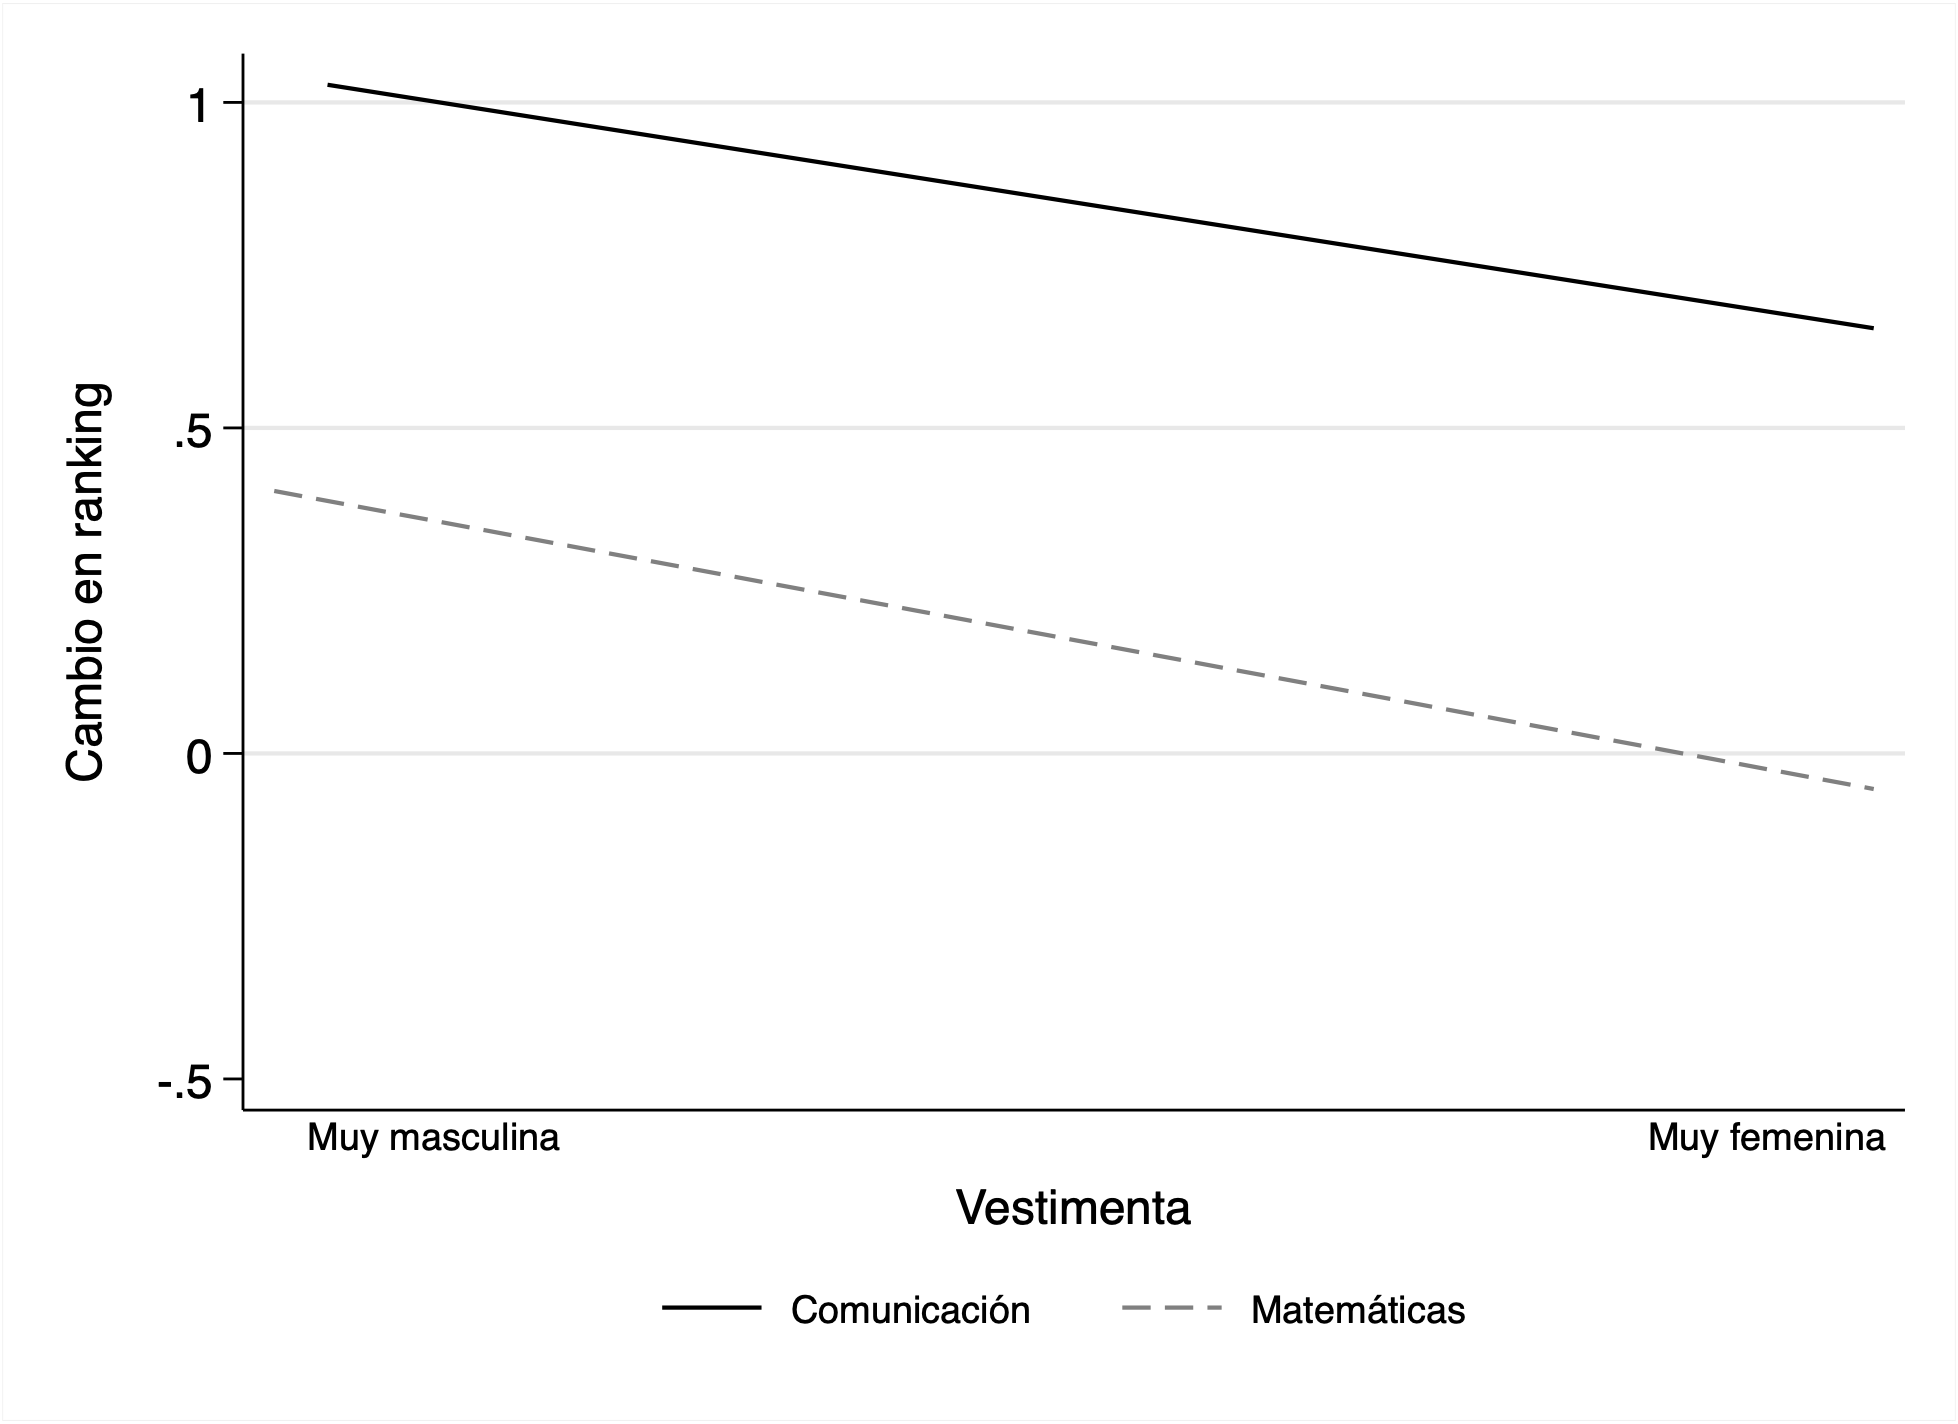
\includegraphics[width=7.8cm]{Images/h3_predicted_rank_score_nocomplier.png}
    \end{subfigure}
\end{figure}
 
Ahora bien, cuando el ranker era de identidad femenina, el efecto de cambiar la vestimenta de muy femenina a muy masculina, condicional a que la habilidad principal eran las matemáticas, es de un aumento de 0.4 d.e. en el \textit{ranking}. Por el contrario, cuando la habilidad principal de sus pares era la comunicación, baja el ranking en 0.08d.e. En resumen, los \textit{rankers} de identidad femenina presentaron una preferencia por trabajar con pares que tenían vestimenta masculina y su habilidad principal era la comunicación, y el tipo de persona con la que estaban menos dispuestos a interactuar era con aquellos que tenían vestimenta muy femenina y su habilidad principal eran las matemáticas. 

Cuando el \textit{ranker} era de identidad masculina, las personas con vestimenta femenina y hábiles comunicándose recibieron el mejor ranking. En esta submuestra, el efecto de pasar de tener una vestimenta muy masculina a tener una muy femenina, cuando la habilidad principal era la comunicación, en está submuestra, es de 0.19d.e. Un efecto tres veces más grande que el de la muestra completa. Por el contrario, cuando la habilidad principal eran las matemáticas, los \textit{rankers} de identidad masculina fueron prácticamente indiferentes de la vestimenta. 

\begin{table}
    \centering
    \caption{Diferencia en \textit{ranking} por combinaciones de expresiones de género y tipo de \textit{ranker}}
    \begin{subtable}{\textwidth}
        \centering
        \caption{Todos}
        \fontsize{9.5}{12}\selectfont {
        \begin{tabular}{cccccc}\hline \hline
                                         &	\multicolumn{2}{c}{\textit{Comunicación}}   &   
                                         &	\multicolumn{2}{c}{\textit{Matemáticas}}	\\ \cmidrule{2-3} \cmidrule{5-6}
                                         &  \textit{Vest. F}    &   \textit{Vest. M}    &   
                                         &  \textit{Vest. F}    &   \textit{Vest. M}    \\ \hline
        \textit{Vest. F \& Comunicación} &	-	                &   0.13                &   
                                         &   0.76               &  	0.37                \\
        \textit{Vest. M \& Matemáticas } &  -0.37	            &   -0.23	            &   
                                         &   0.39               &     -	                \\ \hline\hline
    \end{tabular}}
    \end{subtable}
    \begin{subtable}{\textwidth}
        \centering
        \vspace*{0.5cm}
        \caption{\textit{Ranker} femenino}
        \fontsize{9.5}{12}\selectfont {
        \begin{tabular}{cccccc}\hline \hline
                                         &	\multicolumn{2}{c}{\textit{Comunicación}}   &   
                                         &	\multicolumn{2}{c}{\textit{Matemáticas}}	\\ \cmidrule{2-3} \cmidrule{5-6}
                                         &  \textit{Vest. F}    &   \textit{Vest. M}    &   
                                         &  \textit{Vest. F}    &   \textit{Vest. M}    \\ \hline
        \textit{Vest. F \& Comunicación} &  -	                &   -0.18               &   
                                         &  1.03                &   0.12                \\
        \textit{Vest. M \& Matemáticas } &  -0.12	            &   -0.30	            &   
                                         &  0.91                &   -	                \\ \hline\hline
        \end{tabular}}
    \end{subtable}
    \begin{subtable}{\textwidth}
        \centering
        \vspace*{0.5cm}    
        \caption{Ranker masculino}
        \fontsize{9.5}{12}\selectfont {
        \begin{tabular}{cccccc}\hline \hline
                                         &	\multicolumn{2}{c}{\textit{Comunicación}}   &   
                                         &	\multicolumn{2}{c}{\textit{Matemáticas}}	\\ \cmidrule{2-3} \cmidrule{5-6}
                                         &  \textit{Vest. F}    &   \textit{Vest. M}    &   
                                         &  \textit{Vest. F}    &   \textit{Vest. M}    \\ \hline
        \textit{Vest. F \& Comunicación} &	-	                &   0.43                &   
                                         &  0.49                & 	0.56                \\
        \textit{Vest. M \& Matemáticas}  &  -0.56	            &   -0.13	            &   
                                         &  -0.08               &   -	                \\ \hline\hline
        \end{tabular}}
    \end{subtable}
    \begin{subtable}{\textwidth}
        \centering
        \vspace*{0.5cm} 
        \caption{\textit{Compliers}}
        \fontsize{9.5}{12}\selectfont {
        \begin{tabular}{cccccc}\hline \hline
                                         &	\multicolumn{2}{c}{\textit{Comunicación}}   &   
                                         &	\multicolumn{2}{c}{\textit{Matemáticas}}	\\ \cmidrule{2-3} \cmidrule{5-6}
                                         &  \textit{Vest. F}    &   \textit{Vest. M}    &   
                                         &  \textit{Vest. F}    &   \textit{Vest. M}    \\ \hline
        \textit{Vest. F \& Comunicación} &	-	                &   0.67                &   
                                         &  0.66                & 	0.56                \\
        \textit{Vest. M \& Matemáticas } &  -0.56	            &   0.11	            &   
                                         &  0.10                &    -	                \\ \hline\hline
        \end{tabular}}
    \end{subtable}
    \begin{subtable}{\textwidth}
        \centering
        \vspace*{0.5cm}
        \caption{No \textit{Compliers}}
        \fontsize{9.5}{12}\selectfont {
        \begin{tabular}{cccccc}\hline \hline
                                         &	\multicolumn{2}{c}{\textit{Comunicación}}   &   
                                         &	\multicolumn{2}{c}{\textit{Matemáticas}}	\\ \cmidrule{2-3} \cmidrule{5-6}
                                         &  \textit{Vest. F}    &   \textit{Vest. M}    &   
                                         &  \textit{Vest. F}    &   \textit{Vest. M}    \\ \hline
        \textit{Vest. F \& Comunicación} &	-	                &   -0.39               &   
                                         &  0.70                & 	0.25                \\
        \textit{Vest. M \& Matemáticas } &  -0.25	            &   -0.64	            &   
                                         &  0.46                &   -	                \\ \hline\hline
        \end{tabular}}
    \end{subtable}
    \begin{threeparttable}
    \begin{tablenotes}
    \scriptsize{
    \item Nota: Vest. F corresponde a una vestimenta muy femenina (1.5d.e arriba del promedio) y Vest. M corresponde a una vestimenta muy masculina (1.5d.e abajo del promedio). El valor corresponde a la fila menos la columna. Si el valor es positivo, es porque la combinación de expresiones de género de la fila tiene un mejor ranking que la combinación de la columna. Por ejemplo, una persona con todas vestimenta y habilidad femeninas en promedio está 0.13 puestos más arriba en el ranking que una que tiene una vestimenta femenina y habilidad masculina (Panel (a), la fila superior, segunda columna).}
    \end{tablenotes}
    \end{threeparttable}
    \label{tab:hypothesis_tables}
\end{table}

\begin{result}
Existen diferencias en la disposición a interactuar de \textit{rankers} femeninos y masculinos ante diferentes combinaciones de expresiones de género. 
\end{result}

\begin{table}
    \centering
    \caption{Diferencia en ranking entre género del ranker por combinaciones de expresiones de género}
    \label{tab:Diffs}
    \begin{subtable}{0.49\textwidth}
    \centering
    \caption{Por género del \textit{ranker}}
    \fontsize{9.5}{12}\selectfont {
    \begin{tabular}{ccccc}\hline \hline
          \multicolumn{2}{c}{\textit{Comunicación}} &   
        & \multicolumn{2}{c}{\textit{Matemáticas}}	\\ \cmidrule{1-2} \cmidrule{4-5}
          \textit{Vest. F}  &   \textit{Vest. M}    &   
        & \textit{Vest. F}  &   \textit{Vest. M}    \\ \hline
	      0.05	            &   0.66                &
	    & -0.49             &   0.49                \\ \hline \hline
    \end{tabular}}
    \end{subtable}
    \begin{subtable}{0.49\textwidth}
    \centering
    \caption{Por \textit{compliance} del \textit{ranker}}
    \fontsize{9.5}{12}\selectfont {
    \begin{tabular}{ccccc}\hline \hline
          \multicolumn{2}{c}{\textit{Comunicación}} &   
        & \multicolumn{2}{c}{\textit{Matemáticas}}  \\ \cmidrule{1-2} \cmidrule{4-5}
          \textit{Vest. F}  &   \textit{Vest. M}    &   
        & \textit{Vest. F}  &   \textit{Vest. M}    \\ \hline
	      0.13	            &   -0.93               &
	    & 0.18              &   -0.18               \\ \hline \hline
    \end{tabular}}
    \end{subtable}
    \begin{threeparttable} 
    \begin{tablenotes}
    \scriptsize{
    \item Nota: Vest. F corresponde a una vestimenta muy femenina (1.5d.e arriba del promedio) y Vest. M corresponde a una vestimenta muy masculina (1.5d.e abajo del promedio). En el panel (a) el valor corresponde a la diferencia entre la posición promedio que en la que una persona de identidad femenina a un perfil con esa combinación de expresiones de género y la posición promedio que una persona de identidad masculina le da a ese mismo perfil. En el panel (b) el valor corresponde a la diferencia entre la posición promedio que en la que una persona que es \textit{complier} a un perfil con esa combinación de expresiones de género y la posición promedio que una persona que no es \textit{complier} le da a ese mismo perfil.}
    \end{tablenotes}
    \end{threeparttable}
\end{table}

Por último, hay una diferencia en la manera en la que responden a las combinaciones de expresiones de género los participantes que se adhieren a la norma social con sus expresiones de género y los que no se adhieren. Los participantes que son \textit{compliers} con sus expresiones de género, presentaron una preferencia por trabajar con los pares que eran hábiles comunicándose y que tenían una vestimenta femenina. En el orden de los \textit{compliers}, cuando la habilidad principal era la comunicación, pasar de tener una vestimenta muy masculina a una muy femenina, aumentaba el \textit{ranking} en 0.29d.e. Mientras que, cuando la habilidad principal eran las matemáticas, la diferencia entre el ranking que le daban los \textit{compliers} a sus pares era prácticamente independiente a la vestimenta que tuvieran.

Por la otra parte, cuando la persona que organizaba los perfiles no se adhería a la norma social con sus expresiones de género, estos mostraron una preferencia por trabajar con las personas que presentaban una vestimenta masculina y cuya habilidad principal era la comunicación. Lo que resulta interesante de las elecciones de los \textit{rankers} que no fueron \textit{compliers} es que pareciera que no tuvieron en cuenta la habilidad y la vestimenta conjuntamente. Estos \textit{rankers} prefirieron personas hábiles comunicándose siempre en la misma magnitud que las personas hábiles en matemáticas, independiente de su vestimenta. De igual modo, presentaron una preferencia frente a las personas con vestimenta masculina por encima de las que tenían vestimenta femenina, independiente a la habilidad. 
\begin{result}
Existen diferencias en la disposición a interactuar de \textit{rankers} que se adhieren la norma social con sus expresiones de género y los que no se adhieren, ante diferentes combinaciones de expresiones de género. 
\end{result}